\documentclass[conference,a4paper]{IEEEtran}
\IEEEoverridecommandlockouts
% The preceding line is only needed to identify funding in the first footnote. If that is unneeded, please comment it out.
\usepackage{cite}
\usepackage{amsmath,amssymb,amsfonts}
\usepackage{algorithmic}
\usepackage{graphicx}
\usepackage{textcomp}
\usepackage{xcolor}
\def\BibTeX{{\rm B\kern-.05em{\sc i\kern-.025em b}\kern-.08em
    T\kern-.1667em\lower.7ex\hbox{E}\kern-.125emX}}



\begin{document}

\title{Diffraction of an Electromagnetic Laguerre--Gaussian Beam by the End of a Semi-Infinite Gyrotropic Cylinder}

\author{\IEEEauthorblockN{Vasiliy\,A. Es'kin}
\IEEEauthorblockA{\textit{Department of Radiophysics} \\
	\textit{University of Nizhny Novgorod}\\
	Nizhny Novgorod, Russia \\
	vasiliy.eskin@gmail.com}
\and
\IEEEauthorblockN{Alexander\,V. Kudrin}
\IEEEauthorblockA{\textit{Department of Radiophysics} \\
\textit{University of Nizhny Novgorod}\\
Nizhny Novgorod, Russia \\
kud@rf.unn.ru}

}

\def\f{\phi}
\def\e{\varepsilon}
\newcommand{\cir}[1]{\mathop{#1}\limits^\circ}
\def\r{\rho}
\def\d{\textrm{d}}
\def\o{\omega}
\def\a{\alpha}
\def\b{\beta}
\def\PLG{P_{\rm LG}}

\maketitle

\begin{abstract}
Diffraction of an electromagnetic vortex Laguerre--Gaussian beam by the end of a semi-infinite gyrotropic cylinder located in free space is studied. The forward- and backscattered fields are represented using the eigenfunction expansion technique, and a system of integral equations for the expansion coefficients of the fields in the half-spaces on both sides of the cylinder endface is derived and numerically solved. It is found that for the coaxial incidence of the beam on the cylinder in the case where the narrowest part of the beam cross section coincides with the endface, an electrically thin cylinder scatters the power of the incident beam predominantly to the forward- and backward-propagating continuous-spectrum waves, whereas a relatively small part of the incident-beam power goes to the eigenmodes of the cylinder.
\end{abstract}

\begin{IEEEkeywords}
diffraction, electromagnetic vortex beam, Laguerre--Gaussian beam, gyrotropic cylindrical waveguide
\end{IEEEkeywords}

\section{Introduction}
In recent years, there has been a growing interest in the use of electromagnetic vortex beams. Such beams possess not only the spin angular momentum related to the polarization state and having two values but also the orbital angular momentum, which is associated with the spatial structure of the wavefronts and has an infinite number of values. The properties of such vortex beams are used for manipulation of microparticles, increasing the capacity of radio and optical transmission systems~\cite{b8}, and studies of the laser-plasma interaction for obtaining particle beams with the desired properties~\cite{b9,b10,b11}.

In this work, we study the diffraction of an electromagnetic vortex Laguerre--Gaussian beam by the end of a semi-infinite gyrotropic cylindrical waveguide within the framework of a rigorous electromagnetic formulation. As a medium filling the cylinder, we consider a magnetoplasma in the radio-frequency range and a metamaterial consisting of graphene-sandwiched dielectric disks in the infrared range.


\section{Formulation of the Problem and Basic Equations}
Consider the scattering of a monochromatic $(\sim\exp(i\o t))$ $E$-polarized electromagnetic vortex Laguerre--Gaussian beam with angular frequency $\omega$ by a semi-infinite gyrotropic cylinder of radius $a$ located in the region $z>0$ and surrounded by free space in the case where the symmetry axes of the beam and the cylinder coincide [see Fig.~\ref{fig1}(a)]. It is assumed that the medium in the gyrotropic cylinder is either a cold  magnetoplasma or a metamaterial consisting of graphene-sandwiched dielectric disks, as is shown in Figs.~\ref{fig1}(b) and \ref{fig1}(c). An external static magnetic field ${\bf B}_0$ is taken parallel to the cylinder axis. In this case, the medium inside the cylinder is described by the following dielectric permittivity tensor:
\begin{equation}\label{eq1}
{\hat \varepsilon} =
\left(\begin{array}{ccc}
\varepsilon & -i g& 0 \\
i g & \varepsilon & 0 \\
0 & 0 & \eta \\
\end{array} \right).
\end{equation}
In the case of a cold magnetoplasma, the quantities $\varepsilon$, $g$, and $\eta$ in the radio-frequency range under the condition $\omega\gg \omega_{\rm LH}$, where $\omega_{\rm LH}$ is the lower hybrid resonance frequency, are written as~\cite{Ginzburg1970}
\begin{align}\label{eq2}
&\varepsilon = 1 {-} \frac{{\omega_p^2(\omega {-} i\nu_{e} )}}{{\left[ {{{(\omega {-} {i}\nu_{e} )}^2} {-} \omega_{H}^2} \right]\omega }},\quad g = \frac{{\omega _p^2{\omega_{H}}}}{{\left[ {{{(\omega {-} i\nu_{e} )}^2} - \omega_{H}^2} \right]\omega }},\notag\\
&\eta= 1 {-} \frac{{\omega_p^2}}{{(\omega  - i\nu_{e} )\omega }},
\end{align}
where $\omega_{H}$ and $\omega_p$ are the  gyrofrequency and the plasma frequency of electrons, respectively, and $\nu_{e}$ is the effective electron collision frequency in the plasma. Note that in tensor elements~(\ref{eq2}), we neglected the contribution of ions, which is possible under the condition $\omega\gg\omega_{\rm LH}$.
The Gaussian system of units is used in this paper.


We will also consider the case of an artificial medium in the cylinder, provided that the wavelength $\lambda=2\pi/k_0$ ($k_0=\omega/c$ is the free-space wave
number and $c$ is the speed of light in free space) is much longer than the distance $d$ between the graphene layers in this material. Then it may be considered continuous, and its permittivity tensor can be written in the form (\ref{eq1}) with the elements $\varepsilon$, $g$, and $\eta$ described by the following formulas:
\begin{eqnarray}\label{eq3}
&&\varepsilon  = \tilde \varepsilon  - i \frac{{4\pi }}{{\omega d}}{\sigma _0},\qquad g = \frac{{4\pi }}{{\omega d}}{\sigma _H},\qquad \eta  = \tilde \varepsilon,
\end{eqnarray}
where $\tilde{\varepsilon}$ is the dielectric permittivity of the disks between the graphene layers, and $\sigma_0$ and $\sigma_H$ are the elements of the graphene-layer conductivity tensor
\begin{equation}\label{eq4a}
{\hat \sigma} =
\left(\begin{array}{cc}
{{\sigma _0}}&{{\sigma _H}}\\
{ - {\sigma _H}}&{{\sigma _0}}\\
\end{array} \right).
\end{equation}
The expressions for $\sigma_0$ and $\sigma_H$ can be obtained using the Kubo formula~\cite{Gusynin2007} as
\begin{align}\label{eq1_appA}
&{\sigma_0} {=}  {-} \frac{{{e^2}{\it v}_F^{\rm{2}}\hbar |e{B_0}|}}{{ihc}}2(\hbar \omega {-}i2\Gamma )  \sum\limits_{n = 0}^\infty  {\left[ {\left( {1{-}\frac{{{\Delta ^2}}}{{{M_n}{M_{n{+}1}}}}} \right)} \right.} \nonumber\\
&\!\times\! {\frac{{[{n_F}({M_n}){-}{n_F}({M_{n{+}1}})]{+}[{n_F}({-}{M_{n{+}1}}){-}{n_F}({-}{M_n})]}}{{{{({M_n}{-}{M_{n{+}1}})}^2}{-}{{(\hbar \omega {-}i2\Gamma )}^2}}}} \nonumber\\
&\!\times\! \frac{1}{{{M_{n{+}1}}{-}{M_n}}}{+}\left( {1{+}\frac{{{\Delta ^2}}}{{{M_n}{M_{n{+}1}}}}} \right)\frac{1}{{{M_{n{+}1}}{+}{M_n}}}\nonumber\\
&\!\times\!  \left. {\frac{{[{n_F}({-}{M_n}){-}{n_F}({M_{n{+}1}})]{+}[{n_F}({-}{M_{n{+}1}}){-}{n_F}({M_n})]}}{{{{({M_n}{+}{M_{n{+}1}})}^2}{-}{{(\hbar \omega {-}i2\Gamma )}^2}}}} \right],\nonumber\\
&{\sigma _H} = {-}\frac{{{e^2}{\it v}_F^{\rm{2}}\hbar e{B_0}}}{{hc}} \nonumber\\
&\!\times\! 2\sum\limits_{n = 0}^\infty  {[{n_F}({M_n}){-}{n_F}({M_{n{+}1}})]{-}[{n_F}({-}{M_{n{+}1}}){-}{n_F}({-}{M_n})] } \nonumber\\
&\!\times\! \left[ {\left( {1{-}\frac{{{\Delta ^2}}}{{{M_n}{M_{n{+}1}}}}} \right)} \right.\left( {\frac{1}{{{{({M_n}{-}{M_{n{+}1}})}^2}{-}{{(\hbar \omega {-}i2\Gamma )}^2}}}} \right)\left. \right.\nonumber\\
&+ \left.\left( {1{+}\frac{{{\Delta ^2}}}{{{M_n}{M_{n{+}1}}}}} \right)\left( {\frac{1}{{{{({M_n}{+}{M_{n{+}1}})}^2}{-}{{(\hbar \omega {-}i2\Gamma )}^2}}}} \right) \right],
\end{align}
where
\begin{align}
&{n_F}(x) = 1/\left\{\exp [(x{-}\mu )/({k_B}T)]{+}1\right\},\nonumber\\
&{M_n} = \left({\Delta ^2}{+}2n\hbar |e{B_0}|{\it v}_F^{\rm{2}}{\rm{/}}c\right)^{1/2}\nonumber.
\end{align}
Here, $n_F$ is the Fermi distribution function, $M_n$ is the energy of the $n$th Landau level, $B_0$ is the magnitude of the external magnetic field, $\mu$~is the chemical potential, $T$ is the temperature, $\Gamma$ is the scattering rate, ${\it v}_F$ is the Fermi velocity in graphene, $\Delta$ is the exciton gap, $e$ is the absolute value of an electron charge, and $h$ and $\hbar$ are Planck's constant and the reduced Planck's constant, respectively.

\begin{figure}[h]
	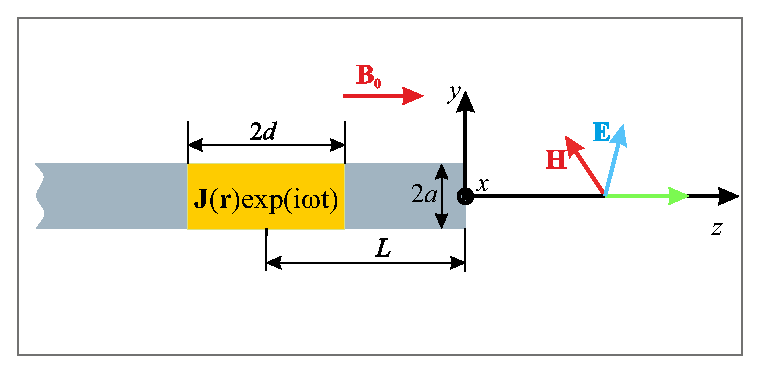
\includegraphics[width=0.9\columnwidth]{fig1.eps}
	\caption{Geometry of the problem.} \label{fig1}
\end{figure}

\section{Solution of the Problem}

It follows from the symmetry of the problem that in the presence of a gyrotropic cylinder, the longitudinal field components in a cylindrical coordinate system ($\rho,\f,z$), with $\exp({i}\omega t)$ time dependence dropped, can be represented as
\begin{equation}\label{eq5}
\begin{bmatrix} {E}_{z;s,m}({\bf r},q)\\ {	H}_{z;s,m}({\bf r},q)\end{bmatrix} = \begin{bmatrix} {E}_{z;s,m}(\rho, q)\\ {H}_{z;s,m}(\rho, q)\end{bmatrix}e^{-i m\f - i k_0
	p_{s}(q)z},
\end{equation}
where $q$ is the transverse wave number in free space, normalized to $k_0$, $m$ is the azimuthal index ($m=0, \pm 1, \pm 2, ...$), the function $p_{s}(q)$ describes the dependence of the normalized (to $k_0$) longitudinal wave number $p_s$ on~$q$ in free space, the subscript~$s$ denotes the wave propagation
direction ($s=-$ and~$s=+$ designate waves propagating in the negative and positive directions of the $z$~axis, respectively), and ${E}_{z;s,m}(\rho, q)$ and~${H}_{z;s,m}(\rho, q)$ are
the functions describing the radial distributions of the longitudinal field components of a wave with the transverse wave number~$q$, the azimuthal index $m$, and the subscript $s$. The functions $p_{\rm +}(q)$ and $p_{\rm -}(q)$ obey the
relation $p_{\rm +}(q)\equiv p(q)= -p_{\rm -}(q)$, where
\begin{equation}\label{eq6}
p(q)=\left(1-q^2\right)^{1/2}.
\end{equation}
It is assumed that ${\rm Im}\,p(q)<0$. For a purely real $p(q)$, the proper branch of this function is chosen with allowance for a minor loss in the medium, which yields the condition ${\rm Re}\,p(q)>0$ in the loss-free case.

The functions $E_{z;s,m}(\rho,q)$  and $H_{z;s,m}(\rho,q)$ satisfy the following equations in the gyrotropic medium~\cite{Kondratev1999}:
\begin{align}
&\displaystyle{ {\hat L}_{m}E_{z;s,m}-k_{0}^{2}\frac{\eta}{\varepsilon}\left(p^{2}_s-\varepsilon\right)E_{z;s,m}{=}{-}{i} k^{2}_{0}\frac{g}{\varepsilon} p_s\, H_{z;s,m} },
\label{eq8}\\
& \displaystyle{ {\hat L}_{m}H_{z;s,m}{-}k_{0}^{2}\left(p^{2}_s +\frac{g^2}{\varepsilon}{-}\varepsilon\right)H_{z;s,m}{=}{i} k^{2}_{0}\frac{g}{\varepsilon}\eta p_s\,E_{z;s,m}},\label{eq9}
\end{align}
where
\begin{equation}
\displaystyle{{\hat{L}}_m =\frac{{\partial}^2}{{\partial}\rho^2} + \frac{1}{\rho}\frac{{\partial}}{{\partial}\rho} - \frac{m^2}{\rho^2} }.\nonumber
\end{equation}
The transverse field components  $E_{\rho;s,m}$, $E_{\f;s,m}$, $H_{\rho;s,m}$, and $H_{\f;s,m}$ can be expressed via the longitudinal components \cite{Kondratev1999}.
% as follows~\cite{Kondratev1999}:
%\begin{eqnarray}
%&& \hspace{-15mm} E_{\rho;s,m} = A
%\left\{ {i} p_sg \frac{m}{\rho}E_{z;s,m}+ {i} p_s(\varepsilon-p_s^2)E_{z;s,m}'+ (\varepsilon-p_s^2)\frac{m}{\rho} H_{z;s,m}+ g H_{z;s,m}'\right\}\!, \label{eq10}\\
%&& \hspace{-15mm} E_{\f;s,m} = A
%\left\{ p_s(\varepsilon-p_s^2)\frac{m}{\rho}E_{z;s,m}+p_sg E_{z;s,m}'- {i} g\frac{m}{\rho}  H_{z;s,m}- {i}(\varepsilon-p_s^2) H_{z;s,m}' \right\}\!,\label{eq11}\\
%&& \hspace{-15mm}H_{\rho;s,m}= A
%\left\{\Big[g^2-\varepsilon(\varepsilon-p_s^2)\Big]\frac{m}{\rho}E_{z;s,m} -p_s^2g E_{z;s,m}' + {i} p_sg\frac{m}{\rho} H_{z;s,m} + {i} p_s(\varepsilon-p_s^2) H_{z;s,m}'\right\}\!,\label{eq12}\\
%&& \hspace{-15mm}H_{\f;s,m} = A
%\left\{{i} p_s^2g\frac{m}{\rho}E_{z;s,m} - {i}\Big[g^2-\varepsilon(\varepsilon-p_s^2)\Big] E_{z;s,m}' + p_s(\varepsilon-p_s^2)\frac{m}{\rho}H_{z;s,m}+ p_sg H_{z;s,m}'\right\}\!,\label{eq12_1}
%\end{eqnarray}
%where $A=k_0^{-1}\left[g^2-{(p_s^2-\varepsilon)}^2\right]^{-1}$ and the prime indicates the derivative with respect to $\rho$.

To obtain equations for the longitudinal field components  and expressions for the corresponding transverse components outside the cylinder, one should put $\varepsilon=1$, $g=0$, and $\eta=1$ in~(\ref{eq8}) and (\ref{eq9}).

Without loss of generality, the vector potential ${{\bf A}^{\!(i)}}\!({\bf r})$ of the incident $E$-polarized vortex Laguerre--Gaussian beam can be written as
\begin{align}
& {{\bf A}^{(i)}}({\bf r}) = {\bf z}_0 A_0 W_n^{(\tilde{m})}(\rho,z) \exp(-{i}\tilde{m}\f-{i}k_0 z).\label{eq10}
\end{align}
Here,
\begin{align}
& W_n^{(\tilde{m})}(\rho,z) = \cos \,\sigma \,K_n^{(\tilde{m})}\left( {\frac{\rho}{b_0} \cos \sigma} \right)\notag\\
&\hspace{5mm}\times \exp \left[ {i\left( {\tilde{m} {+} 2n {+} 1} \right)\sigma  {-} \frac{1}{2}{\left(\frac{\rho}{b_0} \right)^2}\cos\sigma \,{e^{i\sigma }}} \right],\notag
\end{align}
where
\begin{align}
& \sigma  = {\rm arccot}\left( {\frac{{k_0{b_0^2}}}{z}} \right),\quad  K_n^{(\tilde{m})}\left( t \right) = {t^{\tilde{m}}}L_n^{(\tilde{m})}\!\left( {{t^2}} \right).\notag
\end{align}
In the above, $\tilde{m}$ is the topological charge of the beam, $A_0$ is the beam amplitude coefficient, $b_0$ is the radius of the focal spot of the beam, $L_n^{(m)}$ is the associated Laguerre polynomial, and the superscript $(i)$ denotes the incident beam. The vortex Laguerre--Gaussian beam is incident on the waveguide so that the narrowest part of the beam cross section coincides with the endface ($z$ = 0) of the waveguide. Due to the symmetry of the problem, the diffracted field contains only one azimuthal harmonic whose index $m$ is equal to the topological charge of the incident beam, i.e., $m=\tilde{m}$.

The longitudinal components of the backscattered field in the half-space $z<0$ are expanded in terms of the continuous-spectrum waves of free space as
\begin{align}\label{eq15}
&\hspace{-3mm}\left[\!\!\!
\begin{array}{c}
{E_z^{(r)}}\\
{H_z^{(r)}}
\end{array}\!\!\!\right]\!
{=}\!\sum\limits_{\alpha=1}^{2}\!\int_{0}^{\infty}\!\!\!\!\!\!\! a_{m,\alpha}(q)\!\!\left[\!\!\!
\begin{array}{c}
E^{(r)}_{z;-,m,\a}(\rho,q)\\
H^{(r)}_{z;-,m,\a}(\rho,q)
\end{array}\!\!\!\right]\!\!e^{-i m\f+ik_0 p z}{d}q,
\end{align}
where the superscript~$(r)$ denotes the backscattered (reflected) field, and $\alpha=1$ and $\alpha=2$ correspond to the $E$- and $H$-polarized waves, respectively. Then
\begin{align}\label{eq16}
E^{(r)}_{z;s,m,\a}(\rho,q) {=} q J_m(k_0q \rho)\delta_{\a,1},\nonumber\\ H^{(r)}_{z;s,m,\a}(\rho,q) {=} q J_m(k_0q \rho)\delta_{\a,2},
\end{align}
where, $J_m$ is the Bessel function of the first kind of order $m$ and $\delta_{\rm
	\alpha,\beta}$ is the Kronecker delta.

The forward-scattered field in the half-space containing the cylinder ($z>0$) is expanded in terms of the eigenwaves of an infinitely long gyrotropic cylinder, whose parameters coincide with those of the scatterer considered, and consists of the discrete- and continuous-spectrum waves.

Inside the cylinder ($\rho<a$), the functions $E_{z;s,m,\b}(\rho, q)$ and $H_{z;s,m,\b}(\rho, q)$, which describe the longitudinal components of the fields of the continuous-spectrum waves, are re\-pre\-sented as~\cite{Kondratev1999,Eskin2017}
\newcommand{\as}{k_0{q}_k{\rho}}
\newcommand{\az}{\sum_{k=1}^2}
\begin{eqnarray}\label{eq4}
&&\hspace{-7 mm}E_{z;s,m,\b} = \frac{i}{{\eta}} \sum_{k=1}^2
B_{s,m,\b}^{(k)}(q){n}_k{q}_kJ_m(\as),\nonumber\\
&&\hspace{-7 mm}H_{z;s,m,\b} = {-}\sum_{k=1}^2 B_{s,m,\b}^{(k)}(q){q}_kJ_m(\as),
\end{eqnarray}
where $B_{s,m,\b}^{(1)}(q)$ and $B_{s,m,\b}^{(2)}(q)$ are the amplitude coefficients, $q_1$ and $q_2$ are the transverse wave numbers of two normal waves in a gyrotropic medium, which correspond to the same longitudinal wave number $p=p_s(q)$, $s=+$, and the subscript $\b=1,2$ denotes the type of the continuous-spectrum waves (see~\cite{Eskin2017}). Expressions for $q_1$, $q_2$, ${n}_1$, and ${n}_2$ can be found elsewhere~\cite{Kondratev1999}.

In the outer region $\rho >a$, the functions $E_{z;s,m,\b}(\rho, q)$ and $H_{z;s,m,\b}(\rho, q)$ for $z>0$ ($s=+$) can be written in the form
\begin{eqnarray}\label{eq5_1}
&&\hspace{-11 mm} E_{z;s,m,\beta} = q \sum_{k=1}^2 C_{s,m,\beta}^{(k)}(q) H_m^{(k)}(k_0 q\rho)\!,\nonumber\\
&&\hspace{-11 mm} H_{z;s,m,\beta} = q  \sum_{k=1}^2D_{s,m,\beta}^{(k)}(q) H_m^{(k)}(k_0 q\rho)\!,
\end{eqnarray}
where $H_m^{(1)}$ and $H_m^{(2)}$ are the Hankel functions of the first and second kinds of order $m$, respectively, and $C_{s,m,\beta}^{(1)}$, $C_{s,m,\beta}^{(2)}$, $D_{s,m,\beta}^{(1)}$, and $D_{s,m,\beta}^{(2)}$ are the amplitude coefficients which satisfy the following relations:
\begin{align}\label{eq5_2}
&C_{s,m,\beta}^{(1)}(q)= \psi_{s,m,\beta}(q) C_{s,m,\beta}^{(2)}(q),\notag\\
&D_{s,m,\beta}^{(1)}(q)={-} \psi_{s,m,\beta}(q) D_{s,m,\beta}^{(2)}(q).
\end{align}


Recall that the fields of the continuous-spectrum waves satisfy the boundedness conditions at $\rho\to\infty$~\cite{Shevchenko1971,Eskin2017}:
\begin{eqnarray}\label{eq14_1}
\rho^{1/2}\,|{E}_{z;s,m,\b}(\rho, q)|{<}R^{(1)}_m,\,\,\,\,\rho^{1/2}\,|{H}_{z;s,m,\b}(\rho, q)|{<}R^{(2)}_m,
\end{eqnarray}
where $R^{(1)}_m$ and $R^{(2)}_m$ are finite constants.
It follows from (\ref{eq14_1}) that the transverse wave numbers $q$ must be real. In addition, it can be shown that the negative values of $q$ do not give new solutions compared with the positive
$q$ values. Therefore, it suffices to consider only positive transverse wave numbers.
The quantities $\psi_{s,m, 1}(q)$ and $\psi_{s,m, 2}(q)$ in (\ref{eq5_2}) are roots of a quadratic equation that is obtained for $\psi_{s,m, \beta}(q)$ from the requirement that the determinant of a system of linear equations for the coefficients $B_{s,m,\beta}^{(1,2)}$, $C_{s,m,\beta}^{(2)}$, and $D_{s,m,\beta}^{(2)}$ is zero. This system is derived from the conditions of continuity of the field components $E_{\f;s,m,\beta}$, $E_{z;s,m,\beta}$, $H_{\f;s,m,\beta}$, and $H_{z;s,m,\beta}$ on the cylinder surface $\rho=a$ for  purely real values of $q$.

For shortening the notation, the longitudinal filed components of the continuous-spectrum waves will further be written in the following form:
\begin{equation}\label{eq19}
\begin{bmatrix} {E}_{z;s,m,\b} ({\bf r},q)\\
{H}_{z;s,m,\b} ({\bf r},q)\end{bmatrix} =\begin{bmatrix} {E}_{z;s,m,\b}(\rho,q)\\ {H}_{z;s,m,\b}(\rho,q)\end{bmatrix}e^{-i (m\f + k_0 p_{{s}}z)}.
\end{equation}
Accordingly, the longitudinal filed components of the discrete-spectrum waves, i.e., eigenmodes of the gyrotropic waveguide, will be denoted as
\begin{equation}\label{eq13}
\begin{bmatrix} {E}_{z;s,m,n} ({\bf r})\\
{H}_{z;s,m,n} ({\bf r})\end{bmatrix} =\begin{bmatrix} {E}_{z;s,m,n}(\rho)\\ {H}_{z;s,m,n}(\rho)\end{bmatrix}e^{-i (m\f + k_0 p_{{s},m,n}z)},
\end{equation}
where the functions ${E}_{z;s,m,n}(\rho)={E}_{z;s,m,1}(\rho,q_{m,n})$ and ${H}_{z;s,m,n}(\rho)={H}_{z;s,m,1}(\rho,q_{m,n})$ describe the field distribution of an eigenmode with the indices $s$, $m$, and $n$ and the
propagation constant $p_{s,m,n}=p_s(q_{m,n})$, which is defined so that $p_{s,m,n}=p_{m,n}$  for $s=+$ and $p_{s,m,n}=-p_{m,n}$ for $s=-$. Here, the quantities $q_{m,n}$ are roots of the equation $\psi_{s,m,1}(q_{m,n})=0$ and satisfy the condition ${\rm Im}\,q_{m,n} < 0$. %($\psi^{-1}_{s,m,2}(q_{m,n})=0$ in case of ${\rm Im}\,q_{m,n} > 0$).

The fields of the discrete- and continuous-spectrum waves  satisfy the orthogonality relations (see~\cite{Kondratev1999,Shevchenko1971,Eskin2017})
\begin{align}
&\int_0^{2\pi}d\f\int_0^\infty\left( {\bf E}_{s,m,\b}({\bf r},q)\times
\lefteqn{\cir{\phantom{\bf H}}}{\bf H}_{\tilde s,\tilde{m},\tilde{\b}}({\bf r},\tilde q) \right.\nonumber\\
&\hspace{17 mm}\left. - \lefteqn{\cir{\phantom{\bf E}}}{\bf E}_{\tilde
	s,\tilde{m},\tilde{\b}}({\bf r},\tilde q) \times {\bf H}_{s,m,\b} ({\bf r},q)
\right)\cdot{\bf z}_0\,\rho\,d\rho \nonumber\\
&\hspace{17 mm}=\displaystyle{\frac{4\pi}{c}}N_{s,m,\b}(q)\delta(q-\tilde
q)\delta_{s,-\tilde s}\delta_{m,-\tilde m}\delta_{\b,\tilde \b},\label{eq20}\\
&\int_0^{2\pi}d\f\int_0^\infty \left( \begin{bmatrix}{\bf
	E}_{{s},m,n}({\bf r})\\ {\bf E}_{s,m,\b} ({\bf
	r},q)\end{bmatrix}\times \lefteqn{\cir{\phantom{\bf H}}}{\bf H}_{\tilde s, \tilde{m},\tilde n}({\bf r}) \right.\nonumber\\
&\hspace{17 mm}\left. - \lefteqn{\cir{\phantom{\bf E}}}{\bf E}_{\tilde s,\tilde{m},\tilde n} ({\bf
	r}) \times
\begin{bmatrix}{\bf H}_{{s},m,n}({\bf r})\\ {\bf H}_{s,m,\b}({\bf
	r},q)\end{bmatrix}\right)\cdot{\bf z}_0\,\rho\,d\rho\nonumber\\
&\hspace{17 mm}=\begin{bmatrix} \displaystyle{\frac{4\pi}{c}}N_{{s},m,n}\delta_{s,-\tilde s}\delta_{m,-\tilde m}\delta_{n,\tilde n}\\ 0\end{bmatrix},\label{eq21}
\end{align}
which are obtained using Lorentz's theorem in transposed form~\cite{Kondratev1999}. In (\ref{eq20}) and (\ref{eq21}), $\delta(q)$ is the Dirac
function and the circle above the symbols denotes field quantities taken in an auxiliary (``transposed'') medium described by the transposed dielectric tensor~${\hat{\varepsilon}}^{\rm T}$. The
norm of the continuous-spectrum waves of a gyrotropic cylinder is
given by the formula
\begin{align}\label{eq22}
{N}_{s,m,\b}(q){=}&\frac{4 c}{k_0^2}\frac{p_s}{q} (-1)^{m+1}\psi_{s,m,\b}(q)\nonumber\\
&\times \left[\left(C_{s,m,\beta}^{(2)}(q)\right)^{2} {+} \left(D_{s,m,\beta}^{(2)}(q)\right)^{2}\right].
\end{align}
The norm ${N}_{s,m,n}$ of the discrete-spectrum waves can also be written in closed form, but is not given here for brevity.

Thus, the longitudinal components of the forward-scattered field, hereafter marked by the superscript ($t$), are expanded in the region $z>0$ as follows:
\begin{align}\label{eq23}
&\hspace{-4mm}\left[\!\!\!
\begin{array}{c}
{E_z^{(t)}}({\bf r})\\
{H_z^{(t)}}({\bf r})
\end{array}\!\!\!\right]\!\!{=}\!\!\sum\limits_{n} b_{m,n}\!\!\left[\!\!\!
\begin{array}{c}
{E}_{z;+,m,n}^{(t)}(\rho)\\
{H}_{z;+,m,n}^{(t)}(\rho)
\end{array}\!\!\!\right]\!\!e^{-i(m\f + k_0 p_{m,n}z)}\notag\\
&+ \sum\limits_{\beta=1}^{2}\int_{0}^{\infty}\!\!\!b_{m,\beta}(q)\left[\!\!\!
\begin{array}{c}
{E}_{z;+,m,\beta}^{(t)}(\rho,q)\\
{H}_{z;+,m,\beta}^{(t)}(\rho,q)
\end{array}\!\!\!\right]\!\!e^{-i(m\f + k_0 p z)}{d}q.
\end{align}

From the boundary conditions
\begin{eqnarray}\label{eq24}
&&{E}^{(i)}_{\f}+{E}^{(r)}_{\f}={E}^{(t)}_{\f},\quad {H}^{(i)}_{\f}+{H}^{(r)}_{\f}={H}^{(t)}_{\f},\nonumber\\
&&{E}^{(i)}_{\rho}+{E}^{(r)}_{\rho}={E}^{(t)}_{\rho},\quad {H}^{(i)}_{\rho}+{H}^{(r)}_{\rho}={H}^{(t)}_{\rho}
\end{eqnarray}
for the tangential field components at the endface of the cylinder ($z=0$) with allowance for (\ref{eq20}) and (\ref{eq21}), a system of integral equations for the expansion coefficients can be derived in the following form:
\begin{align}
{a}_{m,{\a}}({q}){\tilde N}_{-,m,{\a}}({q})&{+}L_{+ ,-m,\alpha}^{(-)}(q) {=}\sum\limits_{n} {b}_{m,n} {K}^{n,+,m}_{{\a},+,-m}({q})\notag\\
& {+}\sum\limits_{\b=1}^{2}\int_{0}^{\infty}\!\!\!\!{b}_{m,\b}(\tilde{q}){K}^{\b,+,m}_{{\a},+,-m}(\tilde{q},{q}){d}\tilde{q},\label{eq25}\\
{b}_{m,n}{N}_{+,m,n}=&\sum\limits_{\a=1}^{2}\int_{0}^{\infty}\!\!\!\!{a}_{m,\a}(\tilde{q}){K}^{n,-,-m}_{\a,-,m}(\tilde{q}){d}\tilde{q}\notag\\
&+L_{- ,-m,n}^{(+)},\label{eq26}\\
{b}_{m,\b}(q){N}_{+,m,\b}(q)=&\sum\limits_{\a=1}^{2}\int_{0}^{\infty}\!\!\!\!{a}_{m,\a}(\tilde{q}){K}^{\b,-,-m}_{\a,-,m}(q,\tilde{q}){d}\tilde{q}\nonumber\\
&+L_{- ,-m,\b}^{(+)}(q).\label{eq27}
\end{align}
Here, the norm of the continuous-spectrum waves of free space is given by the expression
\begin{eqnarray}\label{eq28}
&& \hspace{-7mm} {\tilde N}_{s,m,{\a}}({q})=(-1)^{m+\alpha}{c}{p_s}/({k_0^2}{q}),
\end{eqnarray}
and the kernels of integral equations (\ref{eq25})--(\ref{eq27}) are given by the formulas
\begin{align}\label{eq11}
\hspace{-1.5mm}{K}^{{n},+,m}_{\a,+,-m}\,({q}){=}&\frac{c}{2} \int_{0}^{\infty}\left({\bf E}^{(t)}_{+,m,{n}}({\bf r})\times{\bf H}^{(r)}_{+,-m,\a}({\bf r},{q})\right.\nonumber\\
&\left. - {\bf E}^{(r)}_{+,-{m},\a}({\bf r},{q})\times{\bf H}^{(t)}_{+,m,{n}}({\bf r})\right)\cdot{\bf z}_0\rho{d}\rho,\nonumber\\
\hspace{-3mm}{K}^{\b,+,m}_{\a,+,-m}\,(q,\tilde{q}){=}&\frac{c}{2}\int_{0}^{\infty}\left({\bf E}^{(t)}_{+,m,\b}({\bf r},q)\times{\bf H}^{(r)}_{+,-m,\a}({\bf r},\tilde{q})\right.\nonumber\\
&\left. - {\bf E}^{(r)}_{+,-{m},\a}({\bf r},\tilde{q})\times{\bf H}^{(t)}_{+,m,\b}({\bf r},q)\right)\cdot{\bf z}_0\rho{d}\rho,\nonumber\\
\hspace{-3mm}{K}^{n,-,-m}_{\a,-,m}\,(\tilde{q}){=}&\frac{c}{2}\int_{0}^{\infty}\left({\bf E}^{(r)}_{-,{m},\a}({\bf r},\tilde{q})\times\lefteqn{\cir{\phantom{\bf H}}}{\bf H}^{(t)}_{-,-m,n}({\bf r})\right.\nonumber\\
&\left. -\lefteqn{\cir{\phantom{\bf E}}}{\bf E}^{(t)}_{-,-m,n}({\bf r})\times{\bf H}^{(r)}_{-,m,\a}({\bf r},\tilde{q}) \right)\cdot{\bf z}_0\rho{d}\rho,\nonumber\\
\hspace{-3mm}{K}^{\b,-,-m}_{\a,-,m}\,(q,\tilde{q}){=}&\frac{c}{2}\int_{0}^{\infty}\left({\bf E}^{(r)}_{-,{m},\a}({\bf r},\tilde{q})\times\lefteqn{\cir{\phantom{\bf H}}}{\bf H}^{(t)}_{-,-m,\b}({\bf r},q)\right.\nonumber\\
&\hspace{-7mm}\left. -\lefteqn{\cir{\phantom{\bf E}}}{\bf E}^{(t)}_{-,-m,\b}({\bf r},q)\times{\bf H}^{(r)}_{-,m,\a}({\bf r},\tilde{q}) \right)\cdot{\bf z}_0\rho{d}\rho.
\end{align}
The other quantities in (\ref{eq25})--(\ref{eq27}), which correspond to the incident beam, are given by the following expressions:
\begin{align}\label{eq12}
 L_{+ ,-m,\a}^{(-)}(q)= & \frac{c}{2}\int\limits_0^\infty \left({\bf{E}}^{(i)}({\bf{r}}) \times {\bf{H}}_{+, - m,\alpha }^{(r)}({\bf{r}},q)\right.\nonumber\\
&\left. -   {\bf{E}}_{+, - m,\alpha }^{(r)}({\bf{r}},q) \times {\bf{H}}^{(i)}({\bf{r}})\right)\cdot{{\bf{z}}_0}\rho d\rho ,\notag\\
L_{- ,-m,n}^{(+)} = & \frac{c}{2}\int\limits_0^\infty \left({\bf{E}}^{(i)}({\bf{r}}) \times \lefteqn{\cir{\phantom{\bf H}}}{\bf{H}}_{-, - m,n }^{(t)}({\bf{r}})\right.\nonumber\\
&\left. -   \lefteqn{\cir{\phantom{\bf E}}}{\bf{E}}_{-, - m,n }^{(t)}({\bf{r}}) \times {\bf{H}}^{(i)}({\bf{r}})\right)\cdot{{\bf{z}}_0}\rho d\rho,\notag
\end{align}
\begin{align}
L_{- ,-m,\b}^{(+)}(q) = & \frac{c}{2}\int\limits_0^\infty \left({\bf{E}}^{(i)}({\bf{r}}) \times \lefteqn{\cir{\phantom{\bf H}}}{\bf{H}}_{-, - m,\b }^{(t)}({\bf{r}},q)\right.\nonumber\\
&\left. -   \lefteqn{\cir{\phantom{\bf E}}}{\bf{E}}_{-, - m,\b }^{(t)}({\bf{r}},q) \times {\bf{H}}^{(i)}({\bf{r}})\right)\cdot{{\bf{z}}_0}\rho d\rho.\notag
\end{align}
Note that all the integrals in (\ref{eq11}) can be evaluated in closed form, which facilitates the search for solutions of the system of integral equations (\ref{eq25})--(\ref{eq27}).


\section{Numerical Results}
To find the expansion coefficients of all waves, the system of integral equations (\ref{eq25})--(\ref{eq27}) was solved using the quadrature method based on Simpson's rules of numerical integration. The upper limits of the integrals in (\ref{eq25})--(\ref{eq27}) were chosen equal to 200. The check of the boundary conditions at the endface of the cylinder and the fulfillment of the energy conservation law were used to control the accuracy of the numerical results.

\subsection{Magnetized Plasma Waveguide}
In the case of a magnetized plasma cylinder, the numerical calculations were performed for the following values of parameters: $\o_{p}/\o_{H} = 12{.}7$, $\o_{H} a/c = 1{.}17$, $\nu_e=0$ and  $\o / \o_H = 0.025$ ($k_0 a= 0.03$). The chosen values can be realized under laboratory conditions in, e.g., the helicon discharge plasma in the rf range~\cite{Kudrin2006}. In this case, the magnetoplasma is resonant and the guiding system supports the propagation of an infinite number of eigenmodes~\cite{Kondratev1999,Kudrin2006}. Note that in this frequency range,  $\e>0$ and $\eta<0$, which is typical of "hyperbolic" materials. The dimensionless radius of the Laguerre--Gaussian beam at the endface $z=0$ is equal to $k_0 b_0 = 2.93$.

Figure~\ref{fig2} shows the partial powers $P_n$ normalized to the power $\PLG$ of the incident Laguerre--Gaussian beam for the first 52 eigenmodes with the radial indices $n\leq 52$ for the beam topological charges $\tilde{m}=1$ and $\tilde{m}=2$. It can be seen in this figure that the most efficient excitation is observed for the modes with $ p_n<P=(\varepsilon-g)^{1/2}=81{.}21$, for which both the helicon and quasielectrostatic parts of the mode fields have the volume structure. In the considered cases, the power going to the eigenmodes amounts to $\sum\limits_{n}P_n\simeq3.4\times 10^{-6} \PLG$ and $\sum\limits_{n}P_n\simeq9.8\times 10^{-8} \PLG$ for $\tilde{m}=1$ and $\tilde{m}=2$, respectively. The power of the incident beam predominantly goes to the forward-scattered waves of the continuous spectrum. The power $P_{\rm cs}^{\rm forw}$ going to these waves amounts to $P_{\rm cs}^{\rm forw} = 0{.}9975 \PLG$ and $P_{\rm cs}^{\rm forw} = 0{.}9917 \PLG$ for $\tilde{m}=1$ and $\tilde{m}=2$, respectively. A significantly lower power $P_{\rm cs}^{\rm back}$ goes to the backscattered waves ($P_{\rm cs}^{\rm back} = 0{.}02 \PLG$ and $P_{\rm cs}^{\rm back} = 0{.}01 \PLG$ for $\tilde{m}=1$ and $\tilde{m}=2$, respectively).


\begin{figure}[h]
	\includegraphics[width=0.9\columnwidth]{fig2.eps}
	\caption{Partial powers $P_n$ normalized to the power $\PLG$ of the Laguerre--Gaussian beam with the topological charges $\tilde{m}=1$ (a) and $\tilde{m}=2$ (b) in the case of a magnetized plasma cylinder.} \label{fig2}
\end{figure}

%m = 1;k_0*a_b= 2.9304;k_0*a_0= 0.0293
%w_p/w_H = 12.6811; w_H * a_0/c = 1.1722; w_0/w_H = 0.025;
%P_beta1 / P_LGBeam = 0.9975
%P_beta2 / P_LGBeam = 2.9381e-08
%sum_modes / P_LGBeam =  3.4338e-06
%P_E / P_LGBeam = 0.0223
%P_H  / P_LGBeam = 2.3984e-07

%m = 2;k_0*a_b= 2.9304;k_0*a_0= 0.0293
%w_p/w_H = 12.6811; w_H * a_0/c = 1.1722; w_0/w_H = 0.025;
%P_beta1 / P_LGBeam = 0.9917
%P_beta2 / P_LGBeam = 8.1892e-09
%sum_modes / P_LGBeam =  9.7812e-08
%P_E / P_LGBeam = 0.01
%P_H  / P_LGBeam = 8.1778e-09


\subsection{Waveguide Filled with a Gyrotropic Metamaterial}
In the case of a waveguide filled with a gyrotropic metamaterial, the numerical calculations were performed for the following values of parameters~\cite{Gusynin2007}: the external magnetic field $B_0=45$~kG, the chemical potential $\mu = 5{.}8\times 10^{-2}$ eV, the temperature $T=10\,{\rm K}$, and the Fermi velocity ${\it v}_F=10^8$ cm/s. We took the scattering rate $\Gamma=0$ and the normalized frequency $\hbar \omega = 0.101$~eV. The dielectric disks between the graphene disks had the thickness $d=10^{-6}$ cm and the dielectric permittivity $\tilde{\varepsilon}=4.5$. The cylinder had radius $a=10^{-4}$ cm ($k_0 a= 0.51$). As in the previous case of a cylinder filled with the magnetoplasma, the metamaterial is resonant and the waveguide supports the propagation of an infinite number of eigenmodes. For this medium, the diagonal elements of the permittivity tensor are such that $\e<0$ and $\eta>0$. The dimensionless radius of the Laguerre--Gaussian beam at $z=0$ was taken equal to $k_0 b_0 = 3.06$.





Figure~\ref{fig3} shows the partial powers $P_n$ normalized to the power $\PLG$ of the incident Laguerre--Gaussian beam for the first 20 eigenmodes with the radial indices $n\leq 20$ if the beam topological charge $\tilde{m}=1$. In the considered case, the total power going to the eigenmodes $(\sum\limits_{n}P_n\simeq 0{.}13 \PLG)$ is comparable with the power of the forward-scattered continuous-spectrum waves ($P_{\rm cs}^{\rm forw} = 0{.}84 \PLG$). Note that the negative values of $p_n$ (see Fig.~3) are related to the fact that the eigenmodes turn out to be backward in this case.
The power $P_{\rm cs}^{\rm back}$ that goes to the backscattered waves amounts to $P_{\rm cs}^{\rm back} = 0{.}012 \PLG$.


{\enlargethispage{-3.1in}}
%m = 1;k_0*a_b= 3.0559; k_0*a_0= 0.5093; 
%a_0 = 1.0000e-04  
%H0 = 4.5 T; w_eV   = 0.1007; GaM_n_eV = 0; m = 1
%P_beta1 / P_LGBeam = 0.7675
%P_beta2 / P_LGBeam = 0.0741
%sum_modes / P_LGBeam =  0.1328
%P_E / P_LGBeam = 0.0067
%P_H  / P_LGBeam = 0.0053

\begin{figure}[h]
	\includegraphics[width=0.9\columnwidth]{fig3.eps}
	\caption{Partial powers $P_n$ normalized to the power $\PLG$ of the Laguerre--Gaussian beam with the topological charge $\tilde{m}=1$ in the case of a cylinder filled with a gyrotropic metamaterial.} \label{fig3}
\end{figure}

\section{Conclusion}
In this paper, we have studied the features of scattering of an $E$-polarized electromagnetic vortex Laguerre--Gaussian beam by the end of a semi-infinite cylinder filled with a magnetoplasma in the radio-frequency range and a gyrotropic metamaterial in the infrared range. It is found that for the coaxial incidence of the beam on the cylinder in the case where the narrowest part of the beam cross section coincides with the cylinder endface, an electrically thin magnetized plasma cylinder scatters the rf power of the incident beam predominantly to the forward- and backward-propagating continuous-spectrum waves. At the same time, a relatively small part of the incident-beam power goes to the eigenmodes of the cylinder. 

In the infrared range, if a cylindrical waveguide is filled with a gyrotropic metamaterial and has a cross-sectional size comparable to the wavelength, the total power going to the discrete-spectrum waves of the cylinder is of the same order of magnitude as the power going to the forward-scattered continuous-spectrum waves.


The results obtained can be useful for diagnostics of media of natural or artificial origin, as well as for developing new devices capable of separating and detecting vortex beams for the needs of telecommunication systems.

\section*{Acknowledgment}

This work was supported by the Russian Science Foundation (project No.~18--72--10046).



\begin{thebibliography}{00}
\bibitem{b8} J. Wang, J.-Y. Yang, I.M. Fazal, A. Nisar, Y. Yan, H. Huang, Y. Ren, Y. Yue, S. Dolinar, M. Tur, and A. E. Willner, ``Terabit free-space data transmission employing orbital angular momentum multiplexing,'' Nature Photon., vol. 6, no. 7, pp. 488--496, June 2012.

\bibitem{b9} A. Denoeud, L. Chopineau, A. Leblanc, and F. Qu\'{e}r\'{e}, ``Interaction of ultraintense laser vortices with plasma mirrors,'' Phys. Rev. Lett., vol. 118, no. 3, p. 033902, January 2017.

\bibitem{b10} L.-X. Hu, T.-P. Yu, Y. Lu, G.-B. Zhang, D.-B. Zou, H. Zhang, Z.-Y. Ge, Y. Yin, and F.-Q. Shao, ``Dynamics of the interaction of relativistic Laguerre--Gaussian laser pulses with a wire target,'' Plasma Phys. Control. Fusion, vol. 61, no. 2, p. 025009, December 2018.

\bibitem{b11} C. Baumann and A. Pukhov, ``Electron dynamics in twisted light modes of relativistic intensity,'' Phys. Plasmas, vol. 25, no. 8, p. 083114, August 2018.

\bibitem{Ginzburg1970}
V.~L. Ginzburg, The Propagation of Electromagnetic Waves in Plasmas. Oxford: Pergamon Press, 1970.

\bibitem{Gusynin2007}
V.\,P. Gusynin, S.\,G. Sharapov, and J.\,P. Carbotte, ``Magneto-optical conductivity in graphene," { J. Phys.: Condens. Matter}, vol. 19, p. 026222, December 2007.

\bibitem{Kondratev1999} I.\,G. Kondrat'ev, A.\,V. Kudrin, and T.\,M. Zaboronkova, Electrodynamics of Density Ducts in Magnetized Plasmas. Amsterdam: Gordon and Breach, 1999.

\bibitem{Eskin2017} V.A. Es'kin and A.V. Kudrin, ``A new method for constructing an orthogonal system of eigenwaves of an open cylindrical waveguide surrounded by an isotropic medium,'' Proc. of PIERS 2017, pp. 843--848, May 2017.

\bibitem{Shevchenko1971} V.~V. Shevchenko, Continuous Transitions in Open Waveguides. Boulder: Golem Press, 1971.

\bibitem{Kudrin2006}
A. V. Kudrin and V. A. Es'kin, ``Whistler wave propagation in a bounded collisional magnetoplasma,'' Phys. Scr., vol. 74, no. 4, pp. 425--438, September 2006.


\end{thebibliography}

\end{document}
